\label{c:Experiments}
The experiments chapter first describes the final experimental pipeline, which is divided into the Stereo Camera Calibration (\autoref{sec:Calibration}) and into the actual reconstruction (\autoref{sec:Reconstruction}) and secondly follows several experimental sessions to point out problems and results which occurred during the tests.

\section{Stereo Camera Calibration}\label{sec:Calibration}
The stereo camera calibration estimates the intrinsic and extrinsic parameters of a set-up of two uncalibrated cameras. The calibration is divided into first capturing image pairs of the checkerboard pattern (\autoref{ssec:PatternSequence}) and then estimating the parameters in the \textit{Stereo Camera Calibrator Toolboox}\index{Stereo Camera Calibrator Toolbox} in MATLAB (\autoref{ssec:estimateStereoParams}). The camera set-up used in the camera calibration must not be changed at all for the rest of the session: the sequence recorded for the actual 3-D reconstruction needs to have the same parameters.

\begin{figure}[htbp]
		\centering
		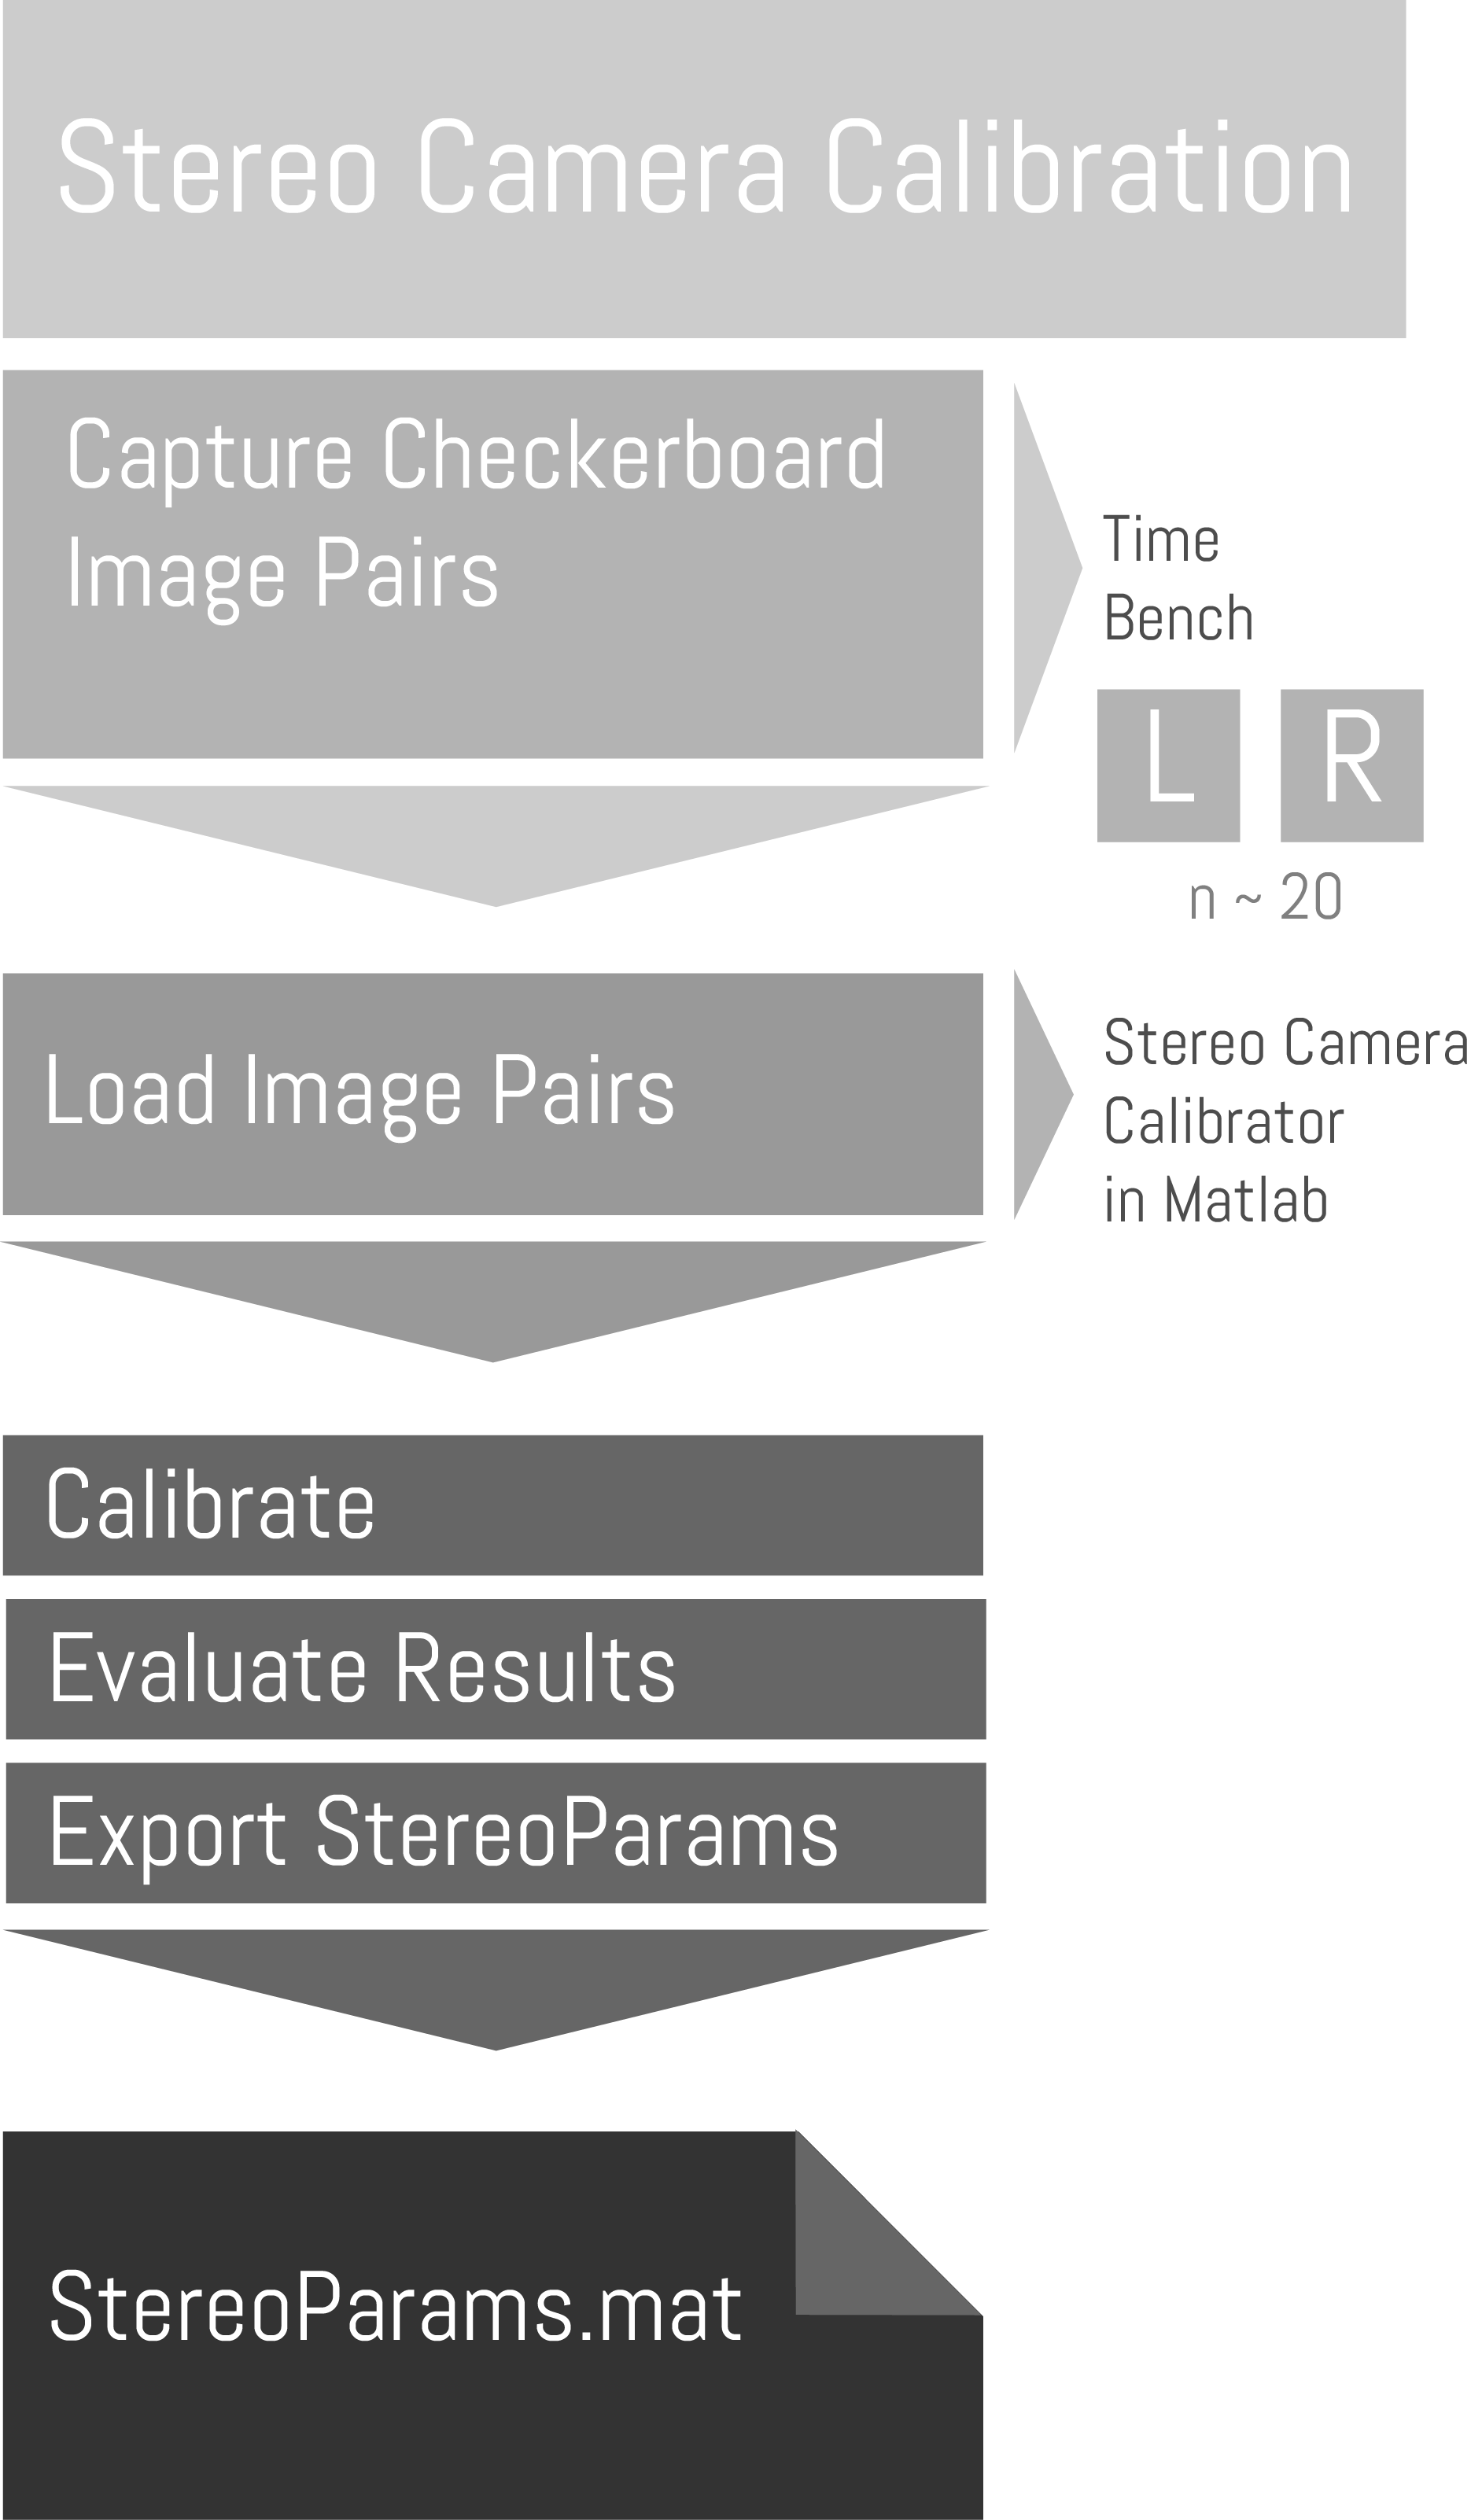
\includegraphics[width=0.7\textwidth]{figures/CameraCalibration}
		\caption[Steps of the stereo camera calibration]{Steps of the stereo camera calibration in TimeBench and in the Stereo Camera Calibrator for MATLAB, using $n$ image pairs.}
		\label{fig:stereoCamCalib}
\end{figure} 

\subsection{Capturing Sequence of Calibration Pattern in TimeBench}\label{ssec:PatternSequence}
The two cameras should be set-up next to each other with little to no rotation. For stereo display (anaglyphic display) the cameras need to be placed about 55 mm apart, which is about the distance between our eyes. Since this thesis does not create stereoscopic displays, the cameras' baseline is set to approximately 19 cm, which is the minimum distance the two cameras can be apart from each other due to the camera bodies.\footnote{Cameras which are placed farther apart from each other resolve in greater reconstruction accuracy.} (\cite{StereoCalib.2016}).  

TimeBench should be only started after the two high-speed cameras have already been connected to the computer, otherwise the cameras may not be recognized by the software. After the hardware was installed (see \autoref{sec:architecture} for the cable set-up), the two cameras need to be dragged into a \textit{synchronization group} and the following configurations are recommended (\autoref{fig:timebanchRecord} shows a screenshot of the connected and synchronized cameras in Timebench): 

\begin{enumerate}[i]
\item Both cameras: set the frame rate to 70 fps\footnote{The smaller frame rate gives more time for positioning the calibration pattern in different angles, since the data amount is decreased to the lower frame rate.}
\item Right camera: check the box \enquote{Is Master} to set the right camera as the synchronization master.
\item Both cameras: set the exposure time slightly shorter than 1/frame rate.
\item Right camera: do not forget to white balance 
\end{enumerate}

\begin{figure}[htbp]
		\centering
		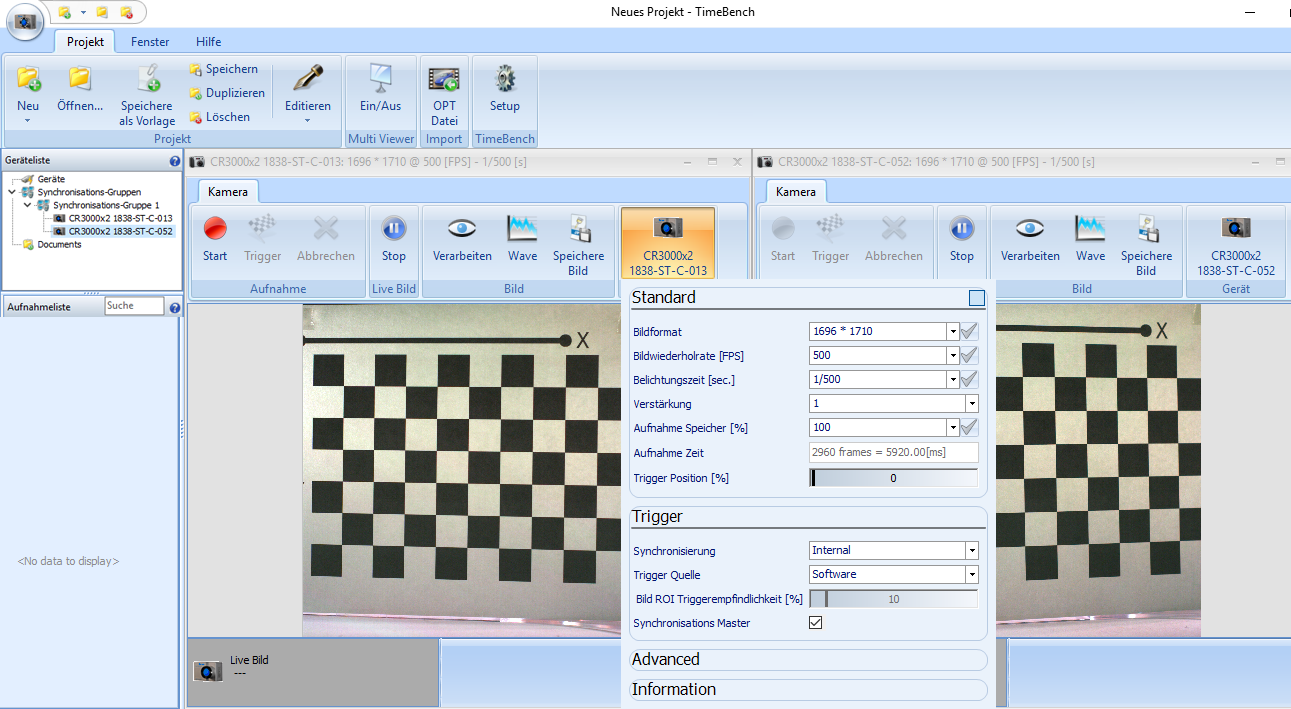
\includegraphics[width=1.0\textwidth]{figures/timebenchRecord}
		\caption[The views of two synchronized cameras and their capturing options in TimeBench]{The views of two synchronized cameras and their capturing options in TimeBench (\textit{source: software TimeBench owned by} \cite{Optronis.2016}).}
		\label{fig:timebanchRecord}
\end{figure}

Once the cameras are synchronized and configured the capturing of the calibration images can begin. The checkerboard pattern should be hold roughly at the same distance the objects will be placed in the actual scene. It needs to be in focus and must be fully visible in the view of both cameras. After starting the capturing sequence by clicking \enquote{Start} in the software and also activating the external trigger, the checkerboard pattern needs to be moved in different angles till the sequence stops. Out of the recorded image sequence 10-20 different image pairs have to be chosen (\autoref{fig:timebenchSequence} shows the timeline with the captured images of a session). Extreme angles are not likely to be detected later in MATLAB (\cite{StereoCalib.2016}).

\subsection{Estimating Stereo Parameters in Matlab}\label{ssec:estimateStereoParams}
The selected set of images pairs of the calibration pattern now need to be loaded into the Stereo Camera Calibration toolbox in MATLAB. They can be added by clicking \textbf{Add images} in the app. In the final experimental architecture the left camera is set as camera one and the right camera as camera two. In this step the correct size of the checkerboard squares are needed, in this case 3 mm. The images then get analyzed by the software, which can take a while depending on the amount and resolution of the set. The result window shows how many stereo pairs were added and how many were rejected, which can be displayed. The rejection can be cause of several reasons, which will be discussed and summarized in \autoref{sec:ExperimentalResults}. The data browser displays a list of all added image pairs, which should be checked whether they are sorted with their correct corresponding partners. Clicking on one pair of images the detected points are displayed in green color and can be checked more closely with the zoom function (\cite{StereoCalib.2016}).

After reviewing the accepted data, the button \textbf{Calibrate} will start the camera calibration. A diagram shows the overall \textbf{reprojection errors} in pixels\index{Reprojection error} from all images, which is the difference between the detected and the reprojected points, as shown in \autoref{fig:ReprojectionError}. The error should not be higher than 1 pixel but are recommended to be below 0.5 pixel. Outliers, which means errors much higher than the acceptable value, can be selected by moving the red horizontal line. The respective images can then be deleted in the data browser. After that \enquote{Calibrate} needs to be clicked again (\cite{StereoCalib.2016}).

\begin{figure}[htbp]
		\centering
		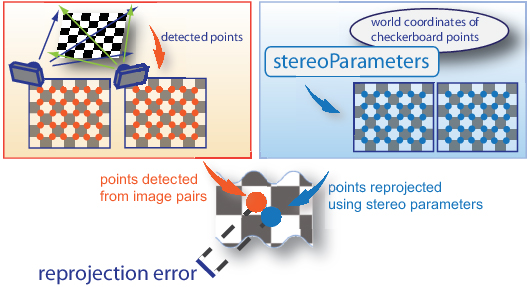
\includegraphics[width=0.9\textwidth]{figures/ReprojectionError}
		\caption[Calculation of the reprojection error]{Calculation of the reprojection error (\textit{source:} \cite{StereoCalib.2016}).}
		\label{fig:ReprojectionError}
\end{figure}

The bottom right window shows the estimated \textbf{extrinsic parameters}\index{Extrinsic camera parameters} in a \textit{camera-centric view}. If the pattern was stationary and the cameras were moved, the plot can be changed to a \textit{pattern-centric view}. This plot should be examined whether the relative poses of the cameras, the baseline and the checkerboard positions are matching the expected positions. 

Another factor to be reviewed is the \textit{rectification}. By clicking on \textbf{Show rectified} in the middle of the screen, the rectified image pair should be shown. If the rectified images are not undistorted and row-aligned the calibration was not accurate enough. This problem is further discussed in the session examples and in the summarized results (\autoref{sec:ExperimentalResults}).

\begin{figure}[htbp]
		\centering
		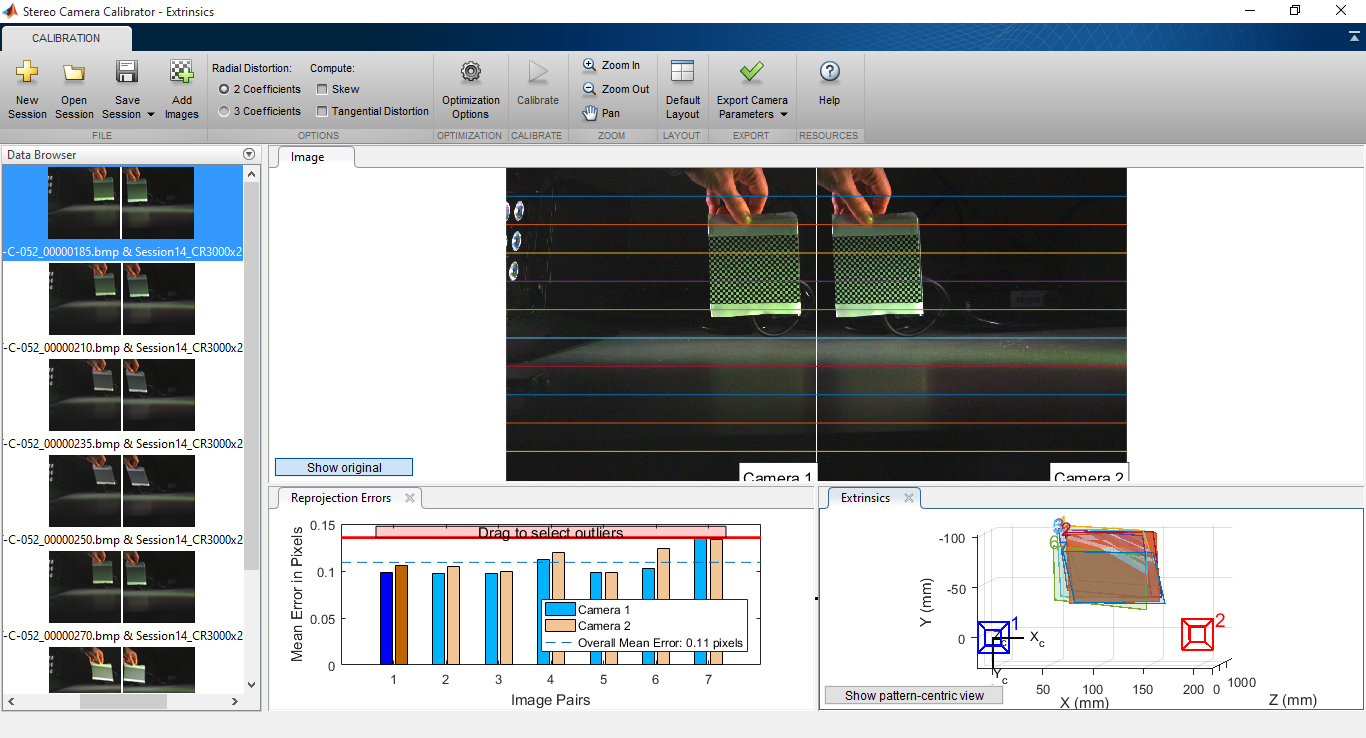
\includegraphics[width=1.0\textwidth]{figures/ExRectified}
		\caption[Calibrated camera system in Matlab]{Calibrated camera system in the Stereo Calibrator with: \textbf{(left)} data browser with set of accepted image pairs; \textbf{(middle)} rectified images of one image pair; \textbf{(bottom left)} reprojection errors; \textbf{(bottom right)} estimated extrinsic parameters.}
		\label{fig:ExRectified}
\end{figure}

The last step is to export the calibrated stereo camera parameters. \textbf{Export camera parameters} creates a \textit{stereoParameters object} in MATLAB's workspace and \textbf{Generate MATLAB script} saves the calibration steps of the session as well.

\subsection{The stereoParameters Object}\label{ssec:stereoParamsObj}
\todo{what does it mean}
\enquote{The object contains the intrinsic and extrinsic parameters of the camera, and the distortion coefficients. You can use this object for various computer vision tasks, such as image undistortion, measuring planar objects, and 3-D reconstruction}(\cite{StereoCalib.2016}).